\chapter{Conclusions}
Since the cancer registration process is partially based on manual
revision, including also the interpretation of the free text in
pathological reports, significant delays in data production and
publication may occur. This weakens data relevance for the purpose of
assessing compliance with updated regional recommended integrated case
pathways, as well as for public health purposes. Improving automated
methods to generate a list of putative incident cases and to
automatically estimate process indicators is thus an opportunity to
perform an up-to-date evaluation of cancer-care quality. In
particular, machine learning techniques like the ones presented in
this work could overcome the delay in cancer case definition by the
cancer registry and allow a powerful tool for timely indicators
computation. The implementation of this procedure could guarantee an
automated and validated instrument to monitor and evaluate diagnostic
and therapeutic pathways.

We analyzed the available data and created different models in order
to implement an automated classification system. We obtained very
encouraging results in classifying cancer cases based on the
interpretation of free text in the data-flow of pathology
reports. This suggests that machine learning methods can be usefully
leveraged in this context. Moreover, we demonstrated that unlabeled
data can 
be effectively used to construct useful word vectors and improve
classification accuracy. 

Our models also have the added value that they can be
utilized to retrieve records adjusting the precision-recall trade-off.

The use of administrative data sources that are up to date combined
with powerful machine learning techniques to automate text
classification is in the interest of the development of a standardized
surveillance system at Regional and National level. Stakeholders and
decision makers need timely and updated indicators to evaluate and
plan healthcare activities. The availability of timely indicators,
routinely and automatically produced, is technically possible. The
main novelty of this work is to show the power of machine learning
techniques applied to the classification of free text pathological
records. This was not yet been systematically implemented in other
Italian cancer registries. This provides a useful monitor tool for
cancer patients pathways, allowing to describe population’s general
health state and to establish public health goals.

The results of the interpretable models can be used to
assist the human classification process on simple records. It can be
used as
a form of text compression, highlighting the most important terms. On
more complex records it can be used to leverage the knowledge of the
model to gain insight on the decision process. To overcome the
limitations of the interpretable
model respect to the general model, in terms of
classification metrics, is it possible to combine the two variants. The
general model can be used to give a more
authoritative classification on the samples while at the same time,
the interpretable model can highlight the same samples.

We compared novel deep learning techniques and more classical models
to pathology records. In this specific context we did not obtain
significant improvements using novel deep learning approaches respect
to classic machine learning methods. Also, the attention methods
usually employed in text classification tasks do not have better
results respect to a more simple max pooling hard attention. Furthermore,
hierarchical models do not work better than plain models. Unsupervised
methods, in particular Word Vectors,
can be used successfully in the
domain of pathological text records. At the best of our knowledge, this
is the first large scale study of deep learning methods applied to
pathology records. Other studies where performed on smaller datasets
with records labeled with less classes.

Regarding the questions in \cref{sec:motivation}, Q1 is answered by
the fact that we implemented several different models to a large scale
dataset of cancer pathology reports. Q2 is answered by the fact that
we used attention models and \ac{bert} in our experiments. To answer
to Q3, from our experiments we have evidence that by using deep learning
methods we do not have a breakthrough compared to classic
\ac{ml} approaches in this specific domain. Regarding Q4, we observe
that hierarchical models are not beneficial in this context. Moreover,
we achieve a little improvement by using attention models, but in
this context a simple max aggregation is equally powerful to the
commonly used attention. About Q5 we observe a successful improvement
when we leverage the unlabeled data, thus we can conclude that
unsupervised techniques can be successfully used in this
context. Finally, in relation to Q6 we studied the potentialities of
interpretable models in the pathology records context.

At the moment it is not possible to use the treated techniques to
completely automate the classification process. The human work is
still needed to get the gold-standard classification where the
supervised models are trained. Moreover, the underlying distribution of
data can drift
with time \cite{klinkenberg2000detecting} (e.g. due to the
introduction of new protocols or terminology), and the most reliable
method to 
deal with this is to periodically update the model retraining
it with fresh labelled data.

Another limit of those techniques is that they can be profitably used
on well represented classes, i.e. common cancer types, but they commit
errors with a rate that is proportional to the rareness of the cancer
cases. The best we can do on this 
front is to use machine learning techniques to fast classify cancer
cases with the awareness of this problem, and rely on the slower human
labelling for sensible cases.

In the future, those techniques can be leveraged to develop a report
classification platform with the double objective of providing an
automated labelling tool, and an aiding tool that helps and
accelerates the human 
labelling process. The automated labelling allows
the implementation of a
fast-speed cancer register that is able to produce updated
statistics at cost of committing errors. The errors can be
controlled 
choosing the classification threshold accordingly to the
recall-precision trade-off --- for this purpose it is possible to use
curves like
\cref{fig:curvesSite,fig:curvesFullSite,fig:curvesType,fig:curvesBehaviour}. The 
aiding tool can employ the interpretable models to implement an
interface similar to \cref{tab:multiAttention1} that can be useful to
accelerate the reading of the report and suggest the most probable
classes.

\begin{figure}
  \centering
  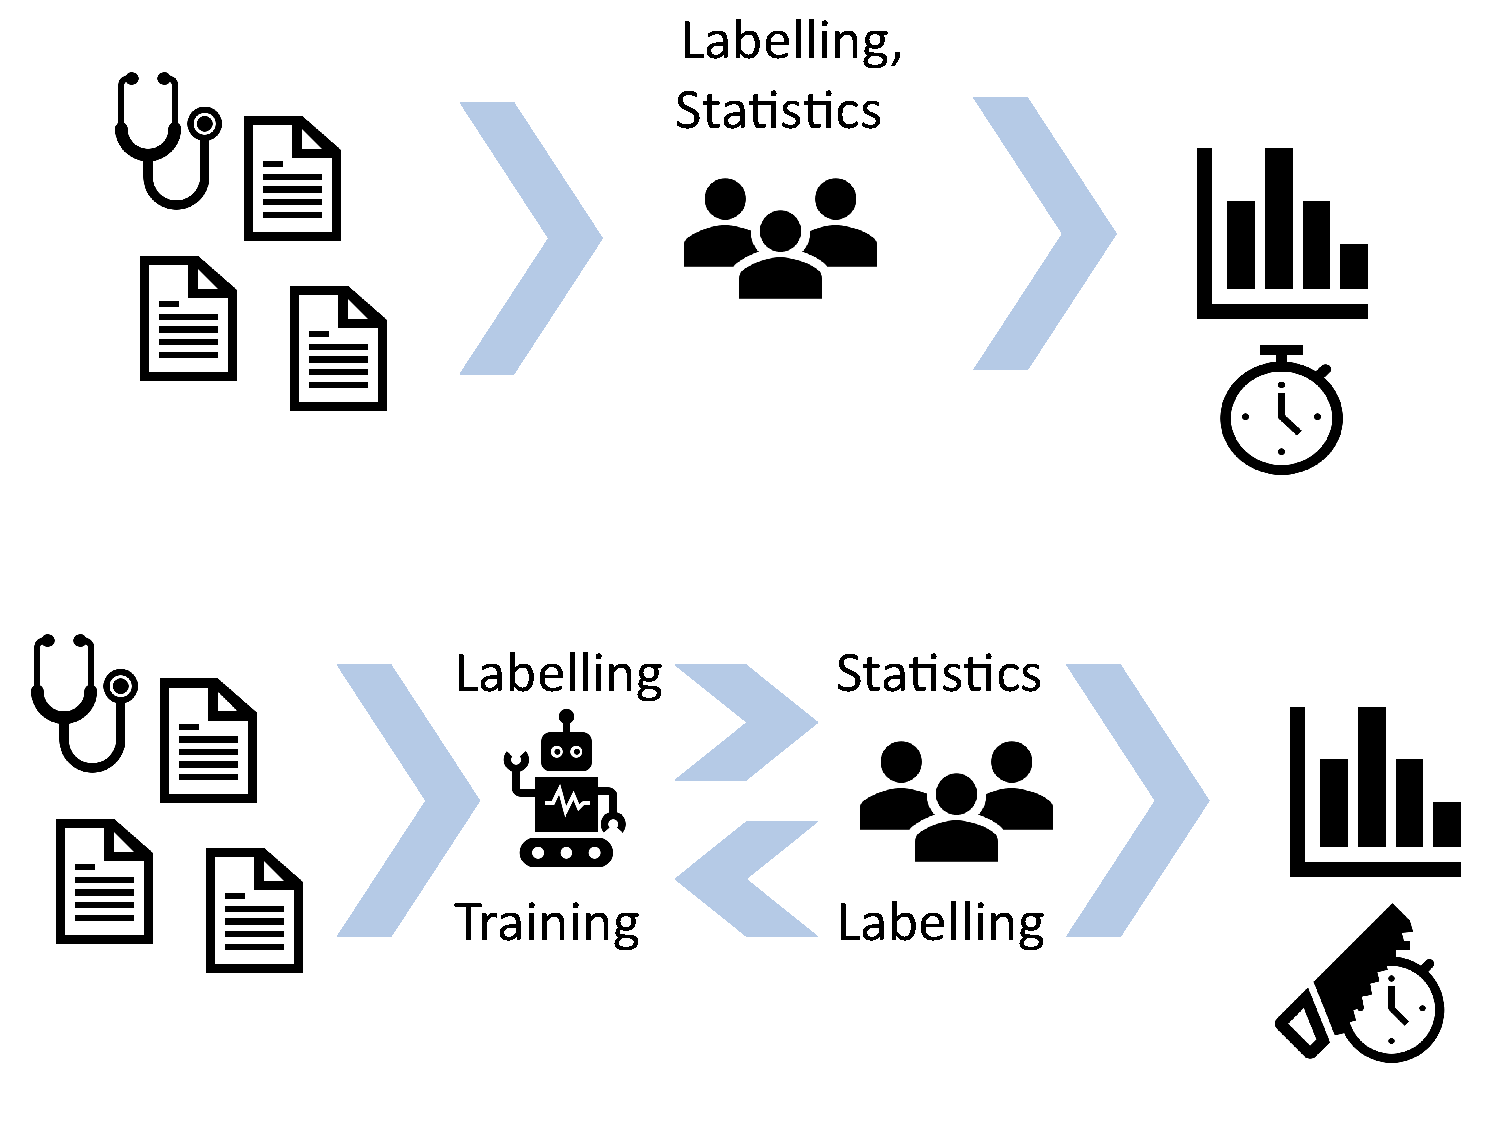
\includegraphics[width=\floatwidth]{img/useCases3.pdf}
  \caption{Current cancer registry workflow (top) and possible
    integration of machine learning methods (bottom).}
  \label{fig:useCases}
\end{figure}
To evaluate a possible use case, consider the current workflow of
cancer registries in the top part of \cref{fig:useCases}. The medical
reports of the competence area are collected and manually labelled by
registry operators. Subsequently the registry calculates useful
statistics on cancer cases. The manual classification of reports
causes a necessary delay on the statistics production.
A possible integration of machine learning methods in this workflow, depicted
in the bottom part 
of \cref{fig:useCases}, is
to use them to automatically label the medical
reports. This labelling can be used to provide fast and
updated statistics on (common) cancer cases. The registry operators
can confirm 
or change the automatic labels providing in this way new data to
train and improve the model in a feedback loop.

A future research direction can be to use multi-task learning
approaches~\cite{caruana1997multitask}, where multiple task can be
solved at the same time. Those 
approaches can be leveraged to improve the classification by sharing
the representations. Another research direction can be to improve the
classification on rare cancer cases using \emph{few-shot learning}
techniques~\cite{wang2019few}. Few-shot learning deals with classes
with few samples, like in our data. \emph{Transfer
  learning}~\cite{pan2009survey} transfers
knowledge learned from a domain where data is available to a domain
where data is scarce. In
\emph{meta-learning}~\cite{hochreiter2001learning} a meta-learner
learns
generic knowledge across tasks and this allows to rapidly generalize a
learner for a specific new task. Both transfer learning and
meta-learning can be used in the context of few-shot learning.

Finally, another research line can focus in the improvement of the
interpretable models. In fact at present time they cannot compete with
other models.

%%% Local Variables:
%%% mode: latex
%%% TeX-master: "thesis"
%%% End:
